\section{Excercise 5}
Cho sơ đồ mạch sau:
\begin{figure}[!htbp]
    \centering
    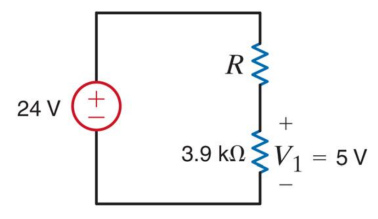
\includegraphics[width=0.5\textwidth]{graphics/ex5/f1.PNG}
    \caption{Sơ đồ mạch điện}
\end{figure}

\begin{enumerate}[label=\alph*.]
    \item Tính R.\\
          Áp dụng KVL:
          \begin{align*}
              V_R & = V - V_{1} = 24 - 5 = 19 \, (\text{V})                  \\
              I   & = \frac{V_{1}}{3,9.10^{3}} = \frac{1}{780} \, (\text{A}) \\
              R   & = \frac{V_{R}}{I} = 14\,820 \, (\Omega)
          \end{align*}
    \item Dùng bảng 2.1 trong slide để chọn điện trở tiêu chuẩn sai số \(10 \%\) cho R. R trong mạch có thể là điện trở đơn hoặc điện trở tương đương của một bộ nhiều điện trở sao cho các điện trở này thỏa mãn giá trị yêu cầu bài toán và có trên thị trường.\\
          Điện trở được chọn: \(15 \, \text{k} \Omega\)
          \begin{figure}[!htbp]
              \centering
              
\includegraphics[width=0.5\textwidth]{graphics/ex5/f2.PNG}
              \caption{Điện trở}
          \end{figure}

          \pagebreak

    \item Dùng điện trở đã chọn ở (b), xác định hiệu điện thế giữa điện trở 3,9 k$\Omega$\\
          Giá trị $V_{1}$ theo điện trở được chọn là:
          \begin{align*}
              V_{1new} = \frac{3,9}{3,9+15}24=\frac{104}{21} \, (\text{V})
          \end{align*}
    \item Tính phần trăm sai số của điện thế $V_{1}$ nếu điện trở tiêu chuẩn ở (b) được dùng.
          \begin{align*}
              \frac{V_{1} - V_{1new}}{V_{1}} = 0,01 \%
          \end{align*}
    \item Xác định công suất của điện trở tiêu chuẩn đã chọn.
          \begin{align*}
              P_{R} = \frac{(24 - V_{1})^{2}}{15.10^{3}} = 0,024 \, (\text{W})
          \end{align*}
\end{enumerate}

\subsection{Mô phỏng}
Kết quả mô phỏng:

\begin{figure}[!htbp]
    \centering
    \begin{subfigure}{.5\textwidth}
        \centering
        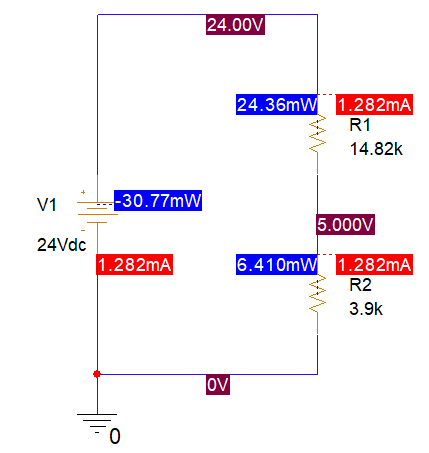
\includegraphics[width=1\linewidth]{graphics/ex5/f3.PNG}
        \caption{Câu a.}
    \end{subfigure}%
    \begin{subfigure}{.5\textwidth}
        \centering
        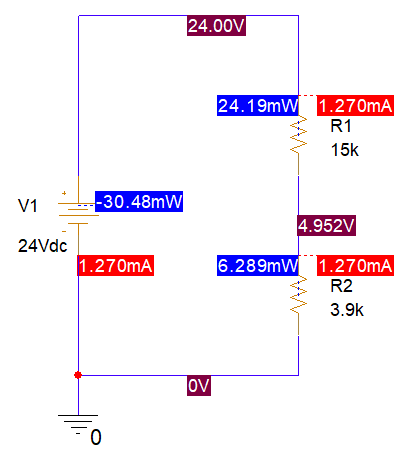
\includegraphics[width=1\linewidth]{graphics/ex5/f4.PNG}
        \caption{Câu b. trở đi}
    \end{subfigure}
    \caption{Mô phỏng mạch điện}
\end{figure}